\section{Kinematic model}
%
\begin{figure}[htb]
    \centering
    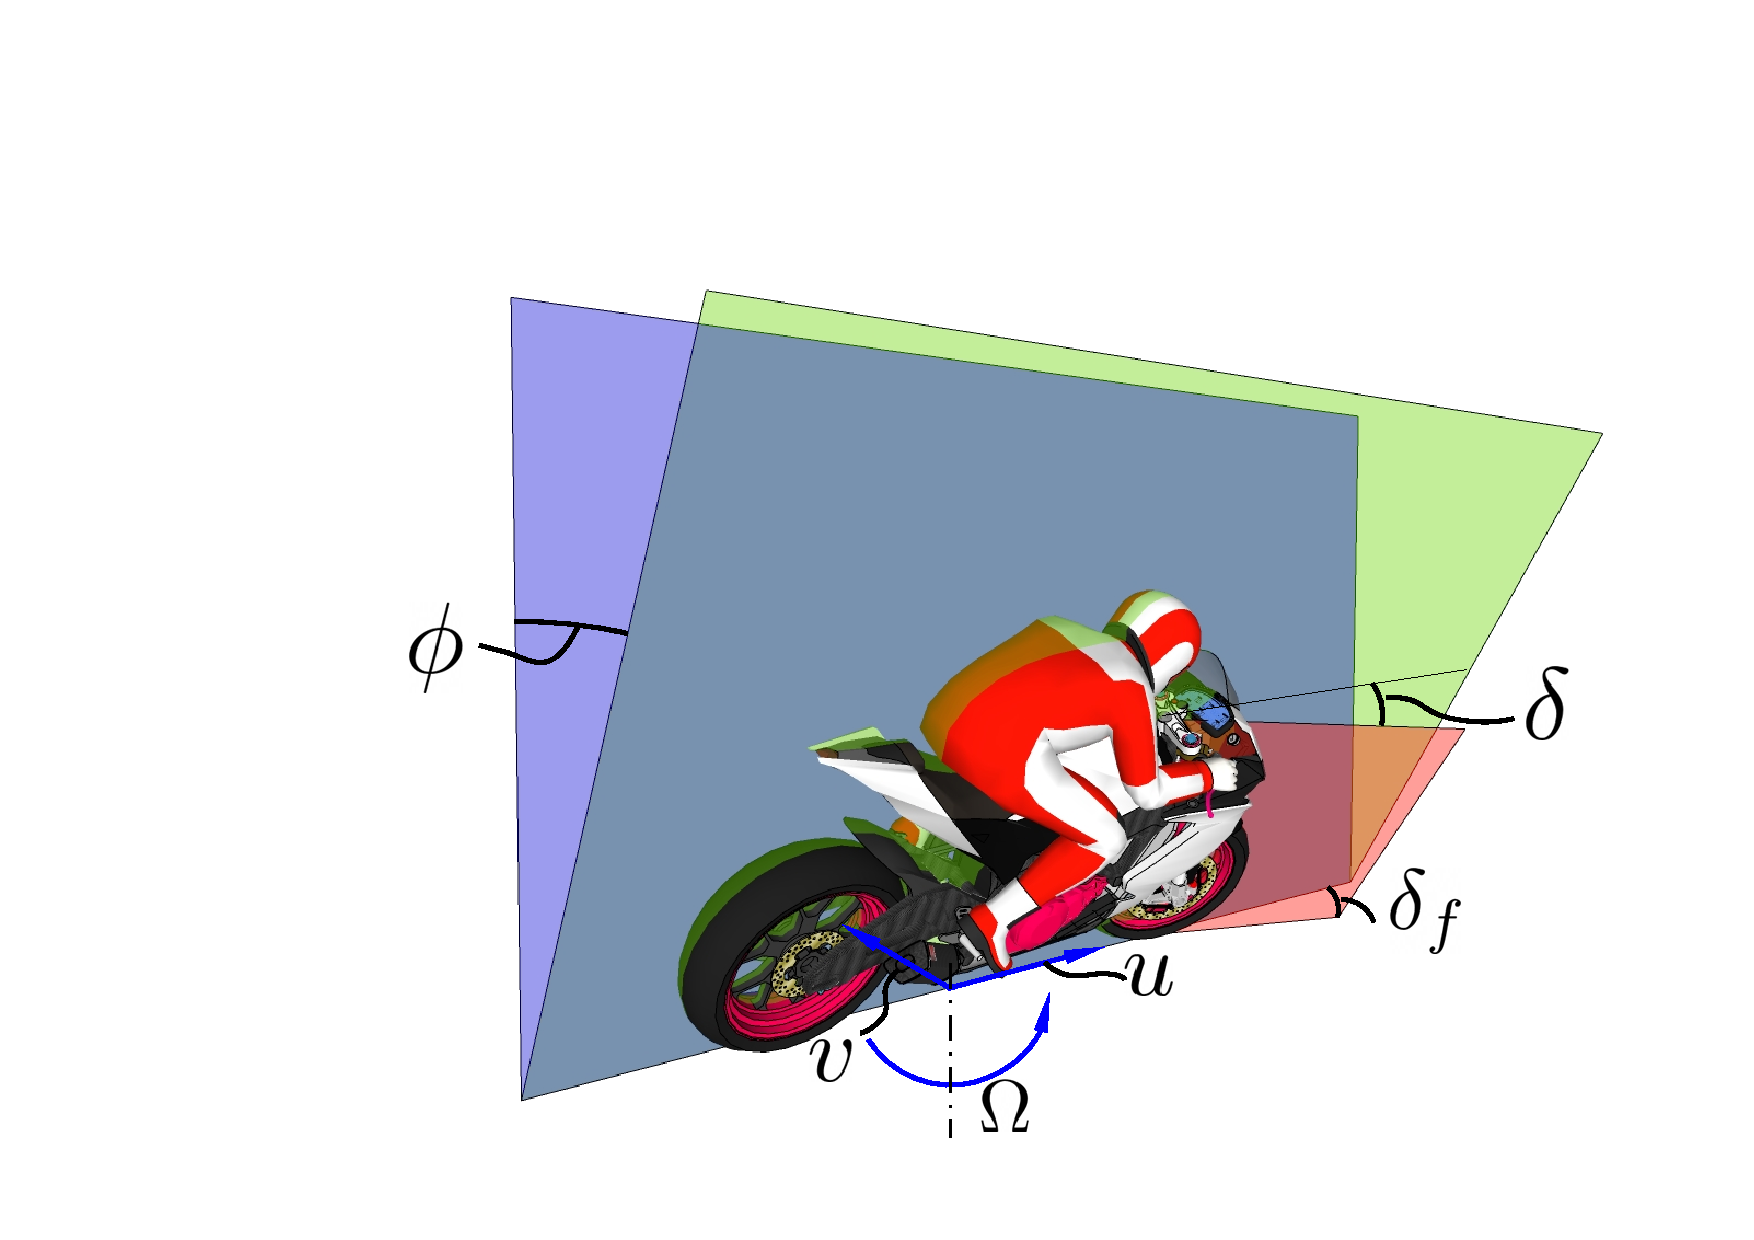
\includegraphics[width=\linewidth]{Coordinates/moto_with_symbols.pdf}
    \caption{Motorcycle representation with some of the Degrees of Freedom}
    \label{fig:MotoLean}
\end{figure}
%
\subsection{Reference frames}
%
A common choice is to start by defining a reference frame in movement with respect to the ground, or fixed, one. This reference frame have in general three linear and three angular velocities. However, for the purpose of this thesis, we consider only planar roads. This means that we need to define the movement of a frame in a plane, therefore only three degrees of freedom are needed (three velocities). The moving reference frame ia addressed as $RF_1$ and has velocities $u(t)$, $v(t)$ and $\Omega(t)$ as can be appreciated from figure \ref{fig:MotoLean}. This set of velocities, also called quasi-coordinates, are suitable to be used later in the definition of curvilinear coordinate. $RF_1$ has the $x$-axis aligned with the direction of motion of the motorcycle. \\
The frame $RF_\phi$ is the reference frame attached to a plane rotated of an angle $\phi(t)$ commonly addressed as rolling angle around the moving $x$-axis and it is obtained recursively multiplying $RF_1$ for a rotation matrix.
%
\begin{equation}
    RF_\phi = RF_1 
    \left[ \begin {array}{cccc} 1&0&0&0\\ \noalign{\medskip}0&\cos
    \left( \phi \left( t \right)  \right) &-\sin \left( \phi \left( t
    \right)  \right) &0\\ \noalign{\medskip}0&\sin \left( \phi \left( t
    \right)  \right) &\cos \left( \phi \left( t \right)  \right) &0
   \\ \noalign{\medskip}0&0&0&1\end {array} \right]   
\end{equation}
%
%
\begin{figure}[htb]
    \centering
    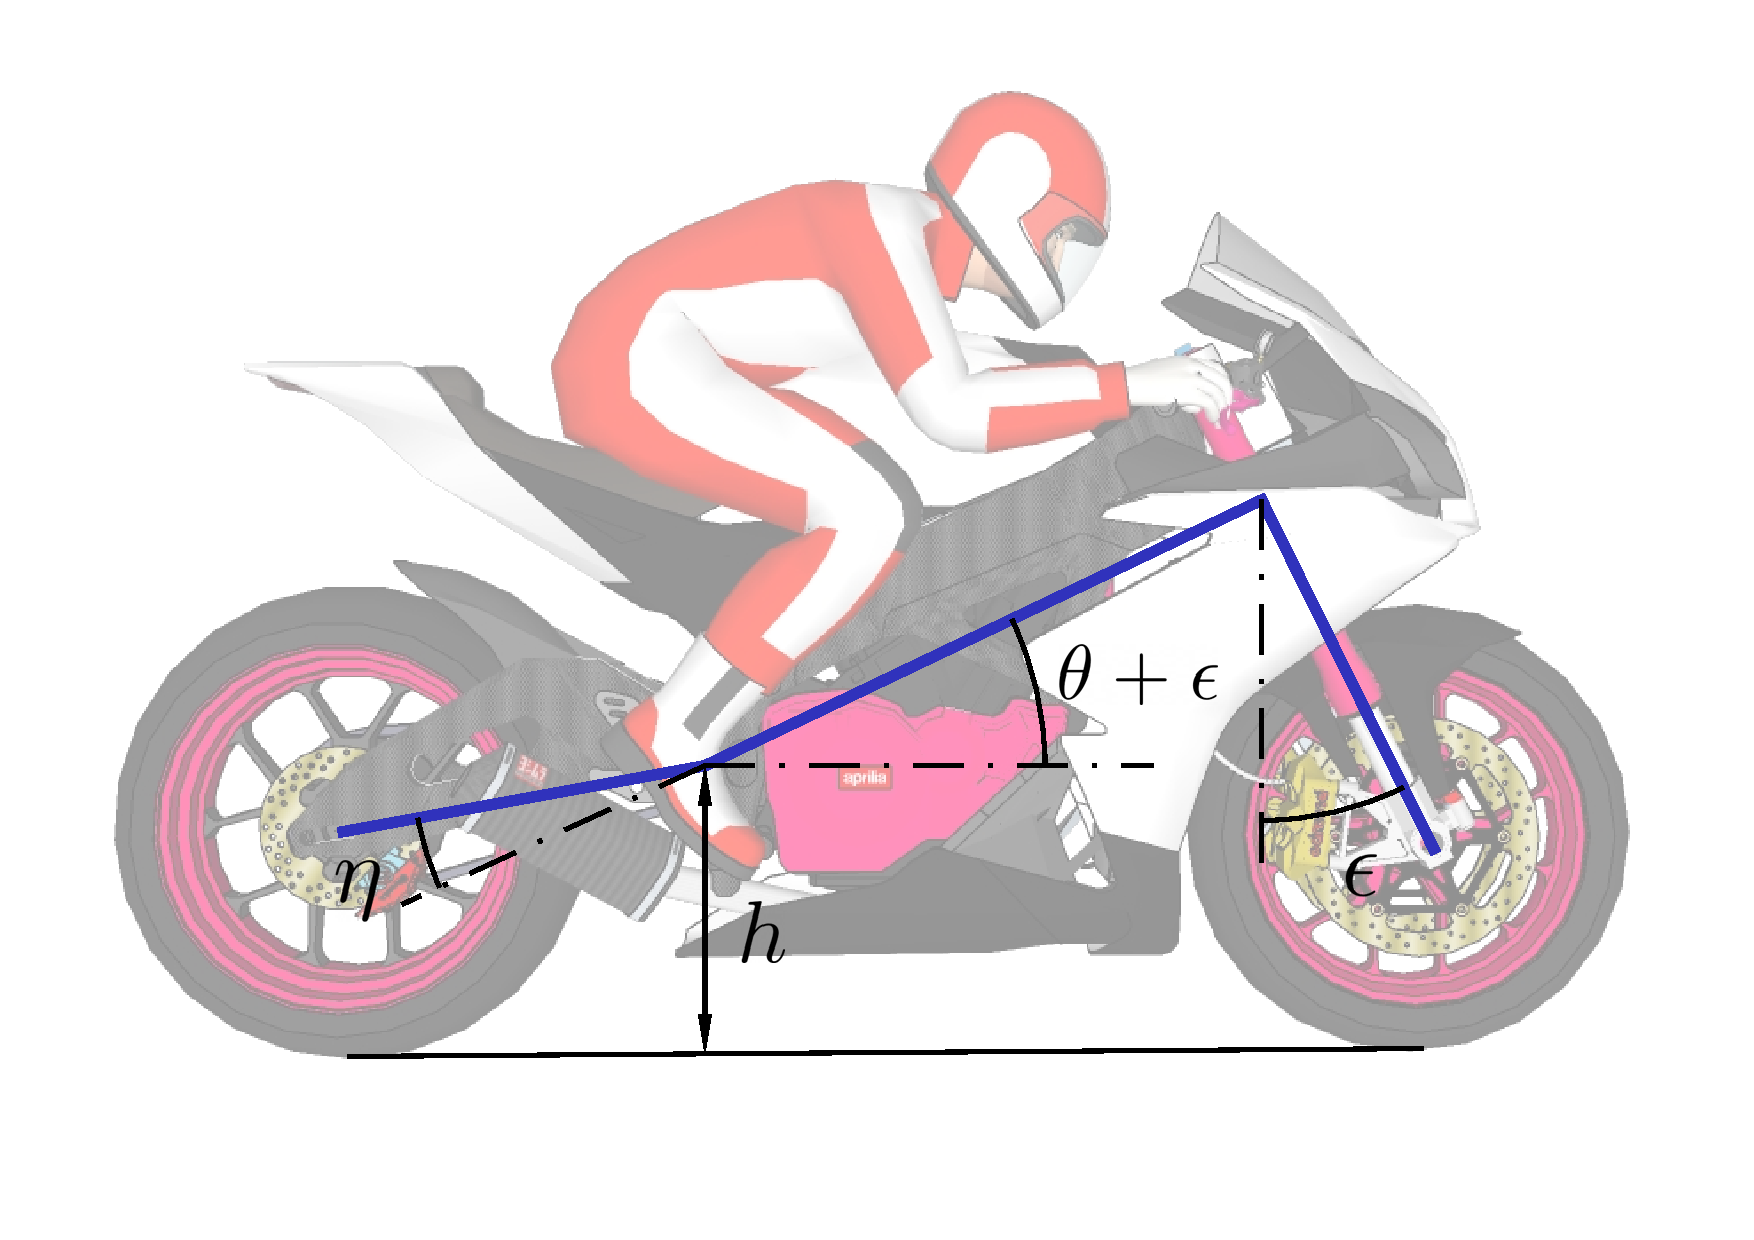
\includegraphics[width=\linewidth]{Coordinates/flankangles.pdf}
    \caption{Motorcycle representation with some of the Degrees of Freedom}
    \label{fig:MotoFlank}
\end{figure}
%
%
Then a reference frame attached to the joint between the swingarm and the rear frame is defined with a translation in the vertical direction of the rolled frame of a certain height $h(t)$ and a rotation around the rolled $y$-axis of an angle $\theta(t)$ plus the caster angle $\epsilon$ (Figure \ref{fig:MotoFlank}). The new frame will be from here addressed as $RF_{Rear}$.
%
\begin{equation}
    RF_{Rear} = RF_\phi 
    \left[ \begin {array}{cccc} \cos \left( \theta \left( t \right) +
    \epsilon \right) &0&-\sin \left( \theta \left( t \right) +\epsilon
    \right) &0\\ \noalign{\medskip}0&1&0&0\\ \noalign{\medskip}\sin
    \left( \theta \left( t \right) +\epsilon \right) &0&\cos \left( 
    \theta \left( t \right) +\epsilon \right) &h \left( t \right) 
    \\ \noalign{\medskip}0&0&0&1\end {array} \right] 
\end{equation}
%
From $RF_{Rear}$ frame one can define the reference frame attached to the swingarm and the one attached to the steering assembly. The first is obtained with a rotation around the $y$-direction of the previous reference frame of a relative angle $eta(t)$ and a translation of the length of the swingarm. The advantage of choosing this relative angle is that there are already define relationship between this rotation an the force of the suspension. The new reference frame is addressed as $RF_\eta$ and will coincide with the centre of the rear wheel.
%
\begin{equation}
    RF_{\eta} = RF_{Rear} 
    \left[ \begin {array}{cccc} \cos \left( \eta \left( t \right) 
    \right) &0&\sin \left( \eta \left( t \right)  \right) &-\cos \left( 
    \eta \left( t \right)  \right) L_{{\it swa}}\\ \noalign{\medskip}0&1&0
    &0\\ \noalign{\medskip}-\sin \left( \eta \left( t \right)  \right) &0&
    \cos \left( \eta \left( t \right)  \right) &\sin \left( \eta \left( t
    \right)  \right) L_{{\it swa}}\\ \noalign{\medskip}0&0&0&1
    \end {array} \right]
\end{equation}
%
The second reference frame, the one attached to the steering assembly has already the $z$-axis with the same direction of the rotation axis of the steer. Therefore, $RF_\delta$ can be obtained with a translation of a fixed quantity in the $x$ direction and a rotation of an angle $\delta(t)$ around the rotation axis $z$. This steering angle is small for racing motorcycle and it is always smaller than $10$ degrees therefore can be linearised from here since the equation of motion are derived using Newton-Euler approach instead of Lagrange.
%
\begin{equation}
    RF_{\delta} = RF_{Rear} 
    \left[ \begin {array}{cccc} 1&-\delta \left( t \right) &0&L_{b}
    \\ \noalign{\medskip}\delta \left( t \right) &1&0&0
    \\ \noalign{\medskip}0&0&1&0\\ \noalign{\medskip}0&0&0&1\end {array}
     \right]    
\end{equation}
%
The reference frame attached to the centre of the front wheel is defined as $RF_{susp}$ and it is obtained with a translation in the negative vertical direction of a fixed quantity $s_{fs}$ plus a time-varying $s_f(t)$ which is the deformation of the suspension and a translation in the $x$ direction of $x_{off}$, an offset always present in the suspension fork.
%
\begin{equation}
    RF_{susp} = RF_\delta 
    \left[ \begin {array}{cccc} 1&0&0&x_{{\it off}}\\ \noalign{\medskip}0
    &1&0&0\\ \noalign{\medskip}0&0&1&-s_{{\it fs}}+s_{f} \left( t \right) 
    \\ \noalign{\medskip}0&0&0&1\end {array} \right] 
\end{equation}
%
In order to have a simplified model one can introduce two new reference frames one for the front and one for the rear wheel starting from $RF_1$. $RF_{FW}$ is defined with a translation of the components $x_f(t)$, $y_f(t)$ and $z_f(t)$ and a rotation of an angle $\delta_f(t)$ around the vertical direction and then one around the new longitudinal direction of angle $\phi_f(t)$. Once again $\delta_f(t)$, which is the steering angle projected to the horizontal plane, is small and can be linearised here.
%
\begin{equation}
    RF_{FW} = RF_1 
    \left[ \begin {array}{cccc} 1&-\delta_{f} \left( t \right) \cos
    \left( \phi_{f} \left( t \right)  \right) &\delta_{f} \left( t
    \right) \sin \left( \phi_{f} \left( t \right)  \right) &x_{f} \left( 
    t \right) \\ \noalign{\medskip}\delta_{f} \left( t \right) &\cos
    \left( \phi_{f} \left( t \right)  \right) &-\sin \left( \phi_{f}
    \left( t \right)  \right) &y_{f} \left( t \right) 
    \\ \noalign{\medskip}0&\sin \left( \phi_{f} \left( t \right)  \right) 
    &\cos \left( \phi_{f} \left( t \right)  \right) &z_{f} \left( t
    \right) \\ \noalign{\medskip}0&0&0&1\end {array} \right] 
\end{equation}
%
The second reference fram $RF_{RW}$ is defined with a translation of the components $x_r(t)$, $y_r(t)$ and $z_r(t)$ and a rotation of an angle $\phi_r(t)$ around the $x$-axis. However since there is no rotation in other planes $\phi_r(t)=\phi(t)$.
%
\begin{equation}
    RF_{RW} = RF_1 
    \left[ \begin {array}{cccc} 1&0&0&-x_{r} \left( t \right) 
    \\ \noalign{\medskip}0&\cos \left( \phi \left( t \right)  \right) &-
    \sin \left( \phi \left( t \right)  \right) &y_{r} \left( t \right) 
    \\ \noalign{\medskip}0&\sin \left( \phi \left( t \right)  \right) &
    \cos \left( \phi \left( t \right)  \right) &z_{r} \left( t \right) 
    \\ \noalign{\medskip}0&0&0&1\end {array} \right]    
\end{equation}
%
Those last two reference frames are attached to the wheels centre. One should also define the reference frame that is spinning by multiplying with a rotation matrix of an angle respectively $\theta_r$ and $\theta_f$.
%
\begin{equation}
    RF_{FWspin} = RF_{FW}
    \left[ \begin {array}{cccc} \cos \left( \theta_{f} \left( t \right) 
    \right) &0&\sin \left( \theta_{f} \left( t \right)  \right) &0
    \\ \noalign{\medskip}0&1&0&0\\ \noalign{\medskip}-\sin \left( \theta_{
    f} \left( t \right)  \right) &0&\cos \left( \theta_{f} \left( t
    \right)  \right) &0\\ \noalign{\medskip}0&0&0&1\end {array} \right]
\end{equation}
%
\begin{equation}
    RF_{RWspin} = RF_{RW}
    \left[ \begin {array}{cccc} \cos \left( \theta_{r} \left( t \right) 
    \right) &0&\sin \left( \theta_{r} \left( t \right)  \right) &0
    \\ \noalign{\medskip}0&1&0&0\\ \noalign{\medskip}-\sin \left( \theta_{
    r} \left( t \right)  \right) &0&\cos \left( \theta_{r} \left( t
    \right)  \right) &0\\ \noalign{\medskip}0&0&0&1\end {array} \right] 
\end{equation}
%
Those angles will not appear directly in the equation of motion. However, their first and second derivative will. Later on $\theta_r$ and $\theta_f$ will be substituted as variable by their derivative, the angular velocities $\omega_r$ and $\omega_f$.\\
One can chose to model the interaction of tyre and asphalt as a pure contact and therefore define two constraints equations, one for each wheel. However, the goal of this thesis is to compute the optimal control and those constraints are not linear and analytically unsolvable. This leads to a system of equation that is a Differential Algebraic Equation (DAE). This can be modelled in two ways. The first is by imposing a penalty in the cost function that minimize those constraints, while the second is deriving the constraints, find an ODE and incorporate the algebraic constrains with a Baumgarte stabilization\cite{baumgarte1972stabilization}. However, those two methods leads to an enlarged problem that should be solved by the optimisation. \\
In this thesis, the chosen solution is to treat the constraints as soft. As did in literature \cite{leonelli2019optimal} the contact is imposed using a force which is proportional to the penetration and the penetration velocity as shown in the next section. For this reason four points are defined in order to get the slip velocities and the penetration of the wheels with the ground. All of those points are defined starting from the reference frame centred in the wheels $RF_{FW}$ and $RF_{RW}$.
The points used for the computation of the slips are:
%
\begin{equation}
P_r =   \left[ \begin {array}{c} 0\\ \noalign{\medskip}0\\ \noalign{\medskip}
-{\it rr}+{\it rtr}-{\frac {{\it rtr}}{\cos \left( \phi \left( t
 \right)  \right) }}\\ \noalign{\medskip}1\end {array} \right] 
\quad \text{in} \; RF_{RW}
\end{equation}
%
\begin{equation}
P_f =   
\left[ \begin{array}{c} 
0\\
0\\ 
-{\it rf}+{\it rtf}-{\frac {{\it rtf}}{\cos \left( \phi_{f} \left( t
 \right)  \right) }}\\
1
\end{array} \right]
\quad \text{in} \; RF_{FW}
\end{equation}
%
While the contact points are defined assuming that the shape of the tyre is a torus. 
%
\begin{equation}
C_r =  \left[ \begin {array}{c} 0\\ 
-\sin \left( \phi
\left( t \right)  \right) {\it rtr}\\ 
-{\it rr}+{
\it rtr}-{\it rtr}\,\cos \left( \phi \left( t \right)  \right)\\ 
1\end {array} \right] 
\quad \text{in} \; RF_{RW}
\end{equation}
%
\begin{equation}
C_f =  \left[ \begin {array}{c} 0\\ 
-\sin \left( \phi_{f}
\left( t \right)  \right) {\it rtf}\\ 
-{\it rf}+{
\it rtf}-\cos \left( \phi_{f} \left( t \right)  \right) {\it rtf}\\
1\end {array} \right] 
\quad \text{in} \; RF_{FW}
\end{equation}
%
Where $rr$, $rf$, $rtr$, $rtf$ are respectively the radius of the rear and front wheel and the radii of the section.
%
\begin{figure}[h!]
    \centering
    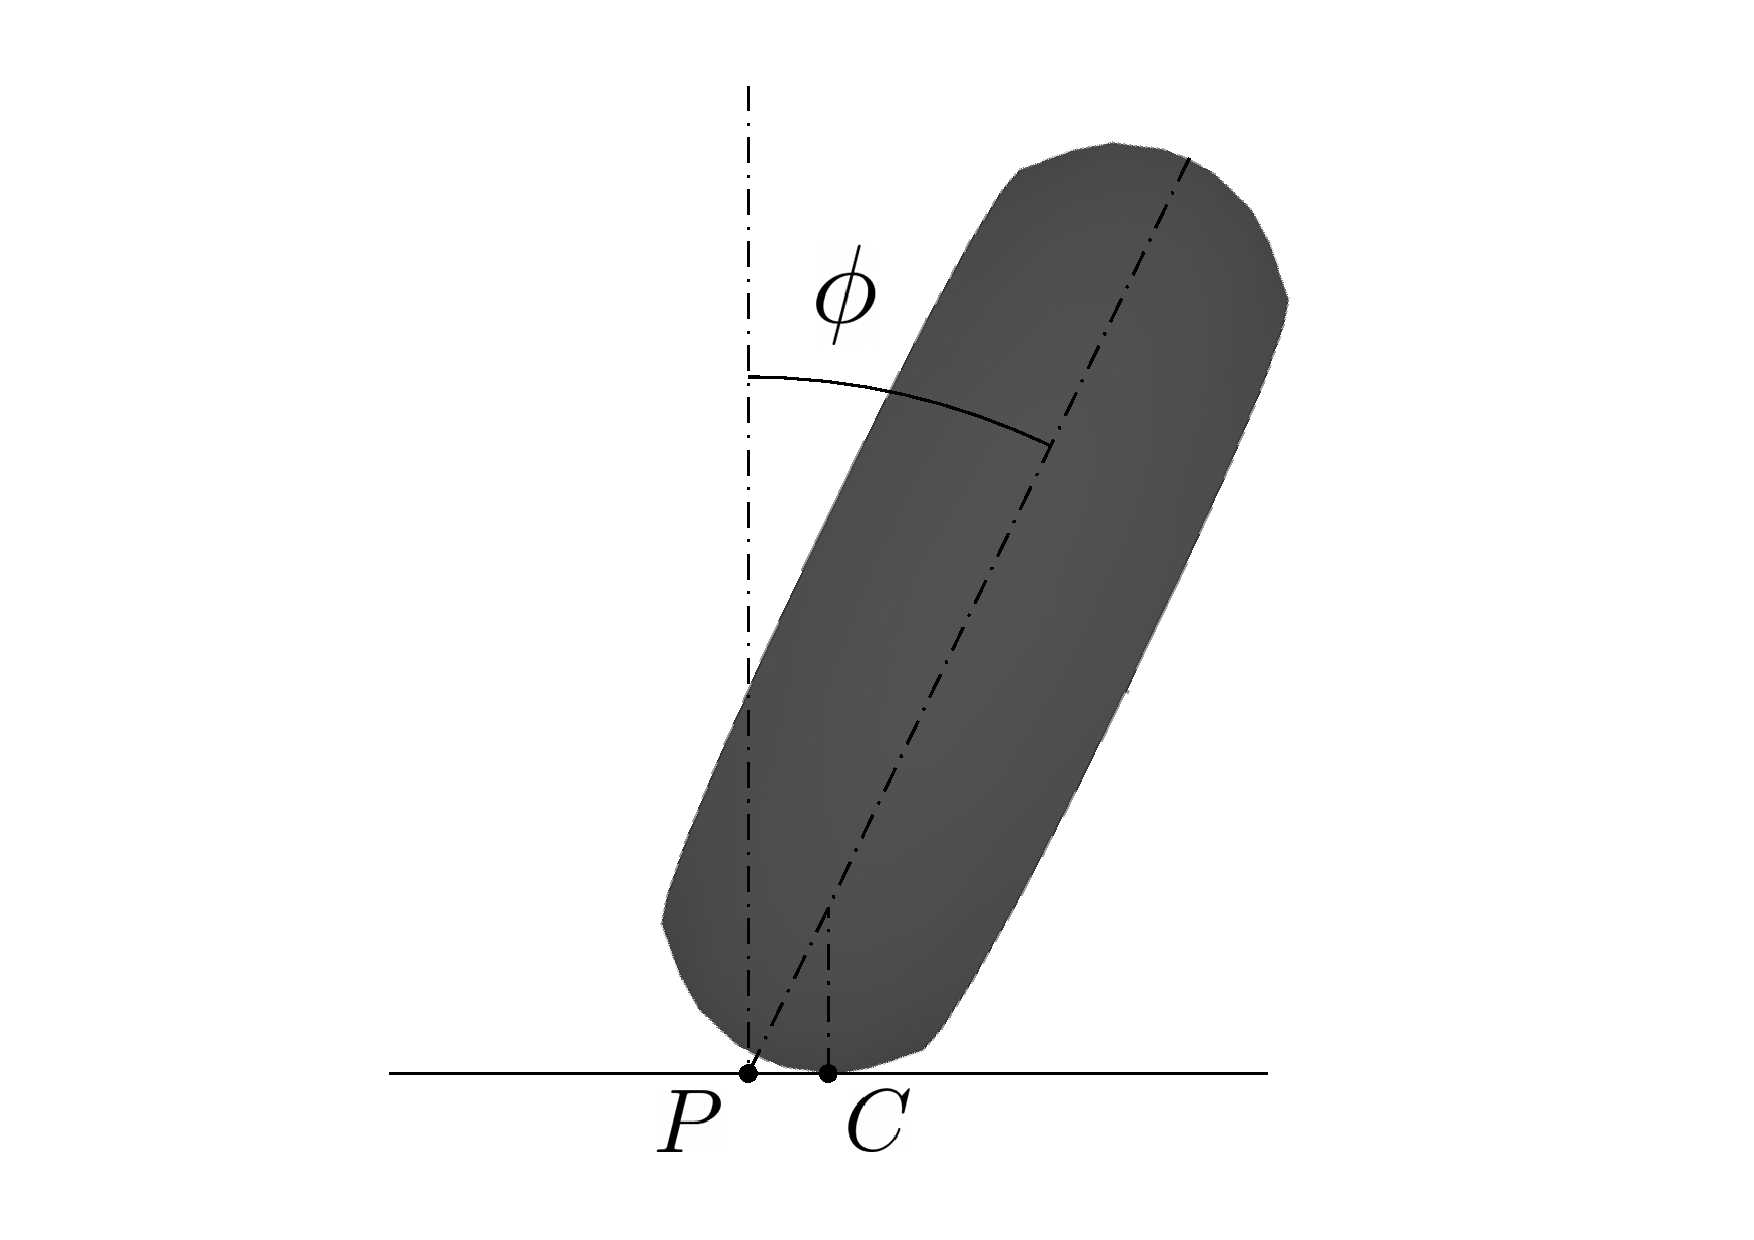
\includegraphics[width=0.5\linewidth]{Coordinates/whellbehind.pdf}
    \caption{Contact point and pont of application of the forces}
    \label{fig:PandC}
\end{figure}
%
\subsection{Kinematic solution}
%
Not all the variable introduced are state variable nor are needed for the final purpose of this thesis. Those have been introduced just to simplify the formulation. However, they can be solved now by imposing some constraints.
$x_f(t)$, $y_f(t)$ and $z_f(t)$ can be solved by imposing that the point of the origin of $RF_{susp}$ is equal to the origin of $RF_{FW}$. This yield 3 algebraic equation in 3 variable.\\
%
\footnotesize
\begin{equation}
    \begin{array}{l} 
        x_{f} \left( t \right) = \left( L_{b}+x_{{
        \it off}} \right) \cos \left( \theta \left( t \right) +\epsilon
         \right) +\sin \left( \theta \left( t \right) +\epsilon \right) 
         \left( s_{{\it fs}}-s_{f} \left( t \right)  \right) \\ 
         \begin{split}
         y_{f} \left( t \right) =\sin \left( \phi \left( t
         \right)  \right)  \left( s_{{\it fs}}-s_{f} \left( t \right) 
         \right) \cos \left( \theta \left( t \right) +\epsilon \right) -\sin
         \left( \phi \left( t \right)  \right)  \left( L_{b}+x_{{\it off}}
         \right) \sin \left( \theta \left( t \right) +\epsilon \right) + \dots 
         \\ \dots +\delta
         \left( t \right) \cos \left( \phi \left( t \right)  \right) x_{{\it 
        off}}-\sin \left( \phi \left( t \right)  \right) h \left( t \right) 
        \end{split} \\ 
        \begin{split}
        z_{f} \left( t \right) =-\cos \left( \phi \left( 
        t \right)  \right)  \left( s_{{\it fs}}-s_{f} \left( t \right) 
         \right) \cos \left( \theta \left( t \right) +\epsilon \right) +\cos
         \left( \phi \left( t \right)  \right)  \left( L_{b}+x_{{\it off}}
         \right) \sin \left( \theta \left( t \right) +\epsilon \right) + \dots
         \\ \dots +\delta
         \left( t \right) \sin \left( \phi \left( t \right)  \right) x_{{\it 
        off}}+\cos \left( \phi \left( t \right)  \right) h \left( t \right) 
        \end{split}
    \end{array}       
\end{equation}
\normalsize
%
The same can be said for the rear wheel. The origin of $RF_{\eta}$ is the same point as the origin of $RF_{RW}$ yielding the following.
%
\footnotesize
\begin{equation}
    \begin{array}{l} x_{r} \left( t \right) = \left( \cos \left( 
        \theta \left( t \right) +\epsilon \right) \cos \left( \eta \left( t
         \right)  \right) +\sin \left( \theta \left( t \right) +\epsilon
         \right) \sin \left( \eta \left( t \right)  \right)  \right) L_{{\it 
        swa}}\\ y_{r} \left( t \right) =-\sin \left( \phi
         \left( t \right)  \right)  \left( L_{{\it swa}}\,\sin \left( \eta
         \left( t \right)  \right) \cos \left( \theta \left( t \right) +
        \epsilon \right) -L_{{\it swa}}\,\cos \left( \eta \left( t \right) 
         \right) \sin \left( \theta \left( t \right) +\epsilon \right) +h
         \left( t \right)  \right) \\ z_{r} \left( t
         \right) =\cos \left( \phi \left( t \right)  \right)  \left( L_{{\it 
        swa}}\,\sin \left( \eta \left( t \right)  \right) \cos \left( \theta
         \left( t \right) +\epsilon \right) -L_{{\it swa}}\,\cos \left( \eta
         \left( t \right)  \right) \sin \left( \theta \left( t \right) +
        \epsilon \right) +h \left( t \right)  \right) \end{array}
\end{equation}
\normalsize
%
The rotation angles $\delta_f(t)$ and $\phi_f(t)$ can be solved as a function of the other states.
The constrain equation can be multiple and each formulation are equal. One can impose orthogonality between reference frames unit vectors or can impose the equality of such vectors. Both ways lead to the following solution.
%
\begin{equation}
\begin{array}{l} \phi_{f} \left(t \right)=-\arcsin \left(
\cos \left(\phi \left(t \right)\right)~\sin \left(\theta \left(t 
\right)+\epsilon \right)~\delta \left(t \right)-\sin \left(\phi \left(
t \right)\right)\right)\\ 
\displaystyle
\delta_{f} \left(t \right)
=\frac{\cos \left(\theta \left(t \right)+\epsilon \right)~\delta 
\left(t \right)}{\sin \left(\phi \left(t \right)\right)~\sin \left(
\theta \left(t \right)+\epsilon \right)~\delta \left(t \right)+\cos 
\left(\phi \left(t \right)\right)}\end{array}
\end{equation} 
%
This can be further simplified keeping in mind that we are considering small angles for $\delta(t)$.
%
\begin{equation}
    \begin{array}{l} \phi_{f} \left( t \right) =-\delta \left( t
    \right) \sin \left( \theta \left( t \right) +\epsilon \right) +\phi
    \left( t \right) \\ 
    \displaystyle
    \delta_{f} \left( t \right) ={
    \frac {\cos \left( \theta \left( t \right) +\epsilon \right) \delta
    \left( t \right) }{\cos \left( \phi \left( t \right)  \right) }}
   \end{array} 
\end{equation}
%
The values obtained will be later substituted in the equation of motion.
%
\subsection{Tyre-Ground penetration}
%
As previously introduced in this thesis, the contact with ground is modelled as a soft constraint using a force which will be a function of the penetration and penetration velocity. The tyre is in this case in equivalent to a spring-damper system.\cite{sharp2004advances,leonelli2019optimal}
The penetration can be obtained by evaluating the vector joining the origin of the $RF_1$ supposed on ground and the two points $C_f$ and $C_r$ at the surface of the torus. The $z$ component of those vectors give a measure of how much the tyre is deformed.
%
\begin{equation}
    \label{eq:penetration}
    \begin{array}{l}
        p_r(t) = - \mathrm{comp\_Z}(O_{RF1}C_r,RF_1)\\
        p_f(t) = - \mathrm{comp\_Z}(O_{RF1}C_f,RF_1)
    \end{array}
\end{equation}
%
The minus sign is present because a positive penetration will generate a positive contact force.
$\mathrm{comp\_Z}$ indicate the component of the vector in the $z$ direction.
The results are not reported here because too long to display.
%
\subsection{Longitudinal and lateral slips}
%
Longitudinal and lateral slips are defined following the definition of practical slip \cite{lot2004motorcycle,pacejka2006tyre}.
The lateral slips are the arctangent of the ratio between longitudinal and lateral velocity of the wheel. 
%
\begin{equation}
    \begin{array}{l}
        \displaystyle \alpha_r(t) = -\arctan( \frac{ \mathrm{comp\_Y}(VP_r,RF_1) }{\mathrm{comp\_X}(VP_r,RF_1)} )\\
        \displaystyle \alpha_f(t) = -\arctan( \frac{\mathrm{comp\_Y}(VP_f,RF_1\cdot R_{\delta_f})}{\mathrm{comp\_X}(VP_f,RF_1\cdot R_{\delta_f})} )
    \end{array}
\end{equation}
%
The longitudinal slip, instead, is defines as the difference between longitudinal velocity and velocity of the point on the wheel divided by the longitudinal velocity.
%
\begin{equation}
    \begin{array}{l}
        \displaystyle \lambda_r(t) = - \frac{( \mathrm{comp\_X,RF_1}(VP_r)  - \omega_r(t) rr )}{\mathrm{comp\_X}(VP_r,RF_1)}\\  
        \displaystyle \lambda_f(t) = - \frac{( \mathrm{comp\_X}(VP_f,RF_1\cdot R_{\delta_f})  - \omega_f(t) rf )}{\mathrm{comp\_X}(VP_f,RF_1\cdot R_{\delta_f})}
    \end{array}
\end{equation}
%
$\omega_r(t)$ and $\omega_f(t)$ are the angular velocities of the wheels also addressed as the time derivative of angles $\theta_r(t)$ and $\theta_f(t)$. $VP_r$ and $VP_r$ are the time derivative of $P_r$ and $P_r$. 
It is important to notice that for the front wheel one should project the velocity vector in the reference frame rotated of the angle $\delta_f(t)$ with respect to the reference frame $RF_1$. 
The results are not reported here because too long to display ($RF_1\cdot R_{\delta_f}$). 
%